\documentclass{article}

\usepackage{../../../uni-notes-eng}
\usepackage{multicol}
\definecolor{back2}{HTML}{ffffff}
\definecolor{text2}{HTML}{000000}
\usepackage{wrapfig}
\usepackage{svg}

\author{Weronika Jakimowicz}
\title{MDM Lista 9}
\date{}

\begin{document}
    \maketitle

    \emph{W języku angielskim krawędzie nazywamy} edges, \emph{więc w anglojęzycznej (a teraz też i międzynarodowej) notacji mielibyśmy $e(G)$ jako oznaczenie ich ilości. Na wykładzie używaliśmy $m(G)$ zamiast $k(G)$ do oznaczenia tej wielkości, co nie ma najmniejszego odniesienia do języka, którym się posługujemy. Z tego też powodu odmawiam używania tej części notacji z wykładu.}

    \subsection*{ZAD. 1.}

    Najpierw przewozimy kozę, a wilka z kapustą zostawiamy na starym brzegu. Potem wracamy z pustą łódką i zabieramy kapustę. Dobijamy do docelowego brzegu, wysadzamy kapustę i zabieramy kozę. Wracamy na startowy brzeg i zostawiamy kozę, po czym szybko zabieramy wilka zanim on złapie kozę. Odstawiamy wilka na brzeg z kapustą, po czym wracamy po kozę i koniec.
    \bigskip

    \podz{sep}
    \bigskip

    Przedstawiamy ten problem za pomocą grafu, którego wierzchołki pokrywają się z wierzchołkami sześcianu. Wierzchołki opiszemy trójkami $(w,g,c)$, gdzie wartości kolejnych współrzędnych to miejsce danej postaci. $w$ będzie oznaczać wilka, $g$ kozę, a $c$ to kapusta. Wartość $0$ oznacza, że dane stworzonko znajduje się na wyjściowym brzegu, a wartość $1$ - na brzegu docelowym.

    \pgraf
        \node (KOZA) at (1, 0) {
            \includesvg[width=15px]{goat}
        };

        \node (WOLF) at (0, 0) {
            \includesvg[width=15px]{wolf}
        };

        \node (CABBAGE) at (2, 0) {
            \includesvg[width=15px]{cabbage}
        };
    \kgraf

    \pgraf
        \node (000) at (0, 0) {(0, 0, 0)};
        \node (100) at (4, 0) {(1, 0, 0)};
        \node (010) at (0, 4) {(0, 1, 0)};
        \node (001) at (2.5, 1.5) {(0, 0, 1)};
        \node (110) at (4, 4) {(1, 1, 0)};
        \node (101) at (6.5, 1.5) {(1, 0, 1)};
        \node (111) at (6.5, 5.5) {(1, 1, 1)};
        \node (011) at (2.5, 5.5) {(0, 1, 1)};

        \draw (000)--(100)--(101)--(111)--(011)--(010)--(000);
        \draw (111)--(110)--(100);
        \draw (110)--(010);
        \draw[color=sep] (000)--(001)--(101);
        \draw[color=sep] (001)--(011);
        
        \draw[very thick, color=def] (000)--(100);
        \draw[very thick, color=def] (000)--(001);
        \draw[very thick, color=def] (011)--(111);
        \draw[very thick, color=def] (110)--(111);
    \kgraf
    
    Zastanówmy się teraz, które krawędzie są na pewno nielegalne. Krawędź $(0,0,0)--(1,0,0)$ oraz $(0,0,0)--(0,0,1)$ zostawiają odpowiednio kapustę lub wilka z kozą, więc ich na pewno nie chcemy użyć. Nie możemy też przejść z $(0,1,1)--(1,1,1)$, bo to znaczy, że dowozimy wilka na brzeg gdzie do tej pory była koza i kapusta. Tak samo ruch $(1,1,0)--(1,1,1)$ implikuje że koza przeżyła z wilkiem sam na sam.

    Zostajemy z dwoma możliwymi ścieżkami od $(0,0,0)$ do $(1,1,1)$:
    $$(0,0,0)--(0,1,0)--(0,1,1)--(0,0,1)--(1,0,1)--(1,1,1),$$
    która jest reprezentacja mojego rozwiązania oraz
    $$(0,0,0)--(0,1,0)--(1,1,0)--(1,0,0)--(1,0,1)--(1,1,1),$$
    gdzie do samotnej kozy zamiast kapusty dowozimy wilka i zabieramy kozę etc.

    \subsection*{ZAD. 2.}

    Rys. 1.
    \smallskip

    Wybierając wierzchołek z dopiskiem $x$ możemy go umieścić na $4$ różnych miejscach. Wiernie pójdzie za nim jego sąsiad z dołu, a jeden wierzchołek z drugiego skrzydełka będzie musiał wybrać jedno z pozostałych dwóch miejsc na skrzydełkach, co daje $2\cdot 4=8$ automorfizmów. Niezależnie od skrzydełek możemy przekręcić lub nie pionową oś, co dodatkowo podwoi nam liczbę automorfizmów, a więc ostatecznie mamy ich
    $$2\cdot 8=16.$$

    Rys. 2.
    \smallskip

    Zaznaczony wierzchołek może przejść na dowolny z tych $8$ które są w grafie. Za nim pójdą jego sąsiedzi, których jest $3$ i możemy im wybrać miejsce na $3!=6$ sposobów. Czyli mamy $8\cdot6=48$ automorfizmów na kostce jako grafie.

    \subsection*{ZAD. 3.}

\begin{center}
\scalebox{.6}
{
    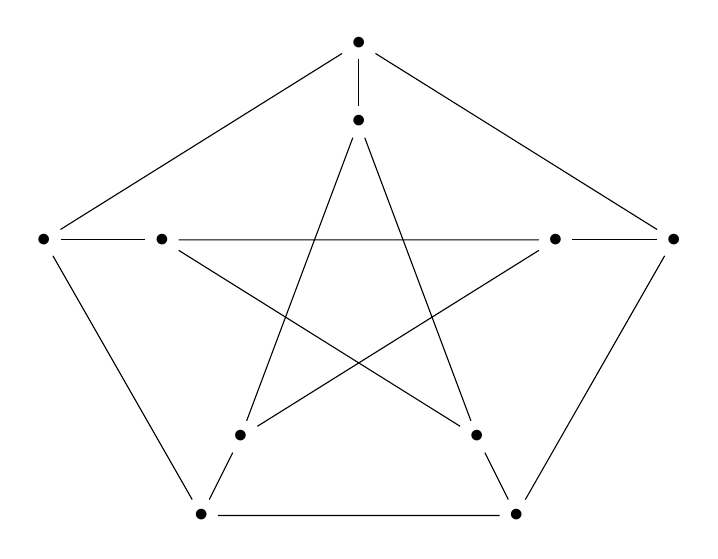
\begin{tikzpicture}
        \node (O1) at (0, 6) {$\bullet$};
        \node (O2) at (4, 3.5) {$\bullet$};
        \node (O5) at (-4, 3.5) {$\bullet$};
        \node (O4) at (-2, 0) {$\bullet$};
        \node (O3) at (2, 0) {$\bullet$};
        \draw (O1)--(O2)--(O3)--(O4)--(O5)--(O1);
        \node (I1) at (0, 5) {$\bullet$};
        \node (I2) at (2.5, 3.5) {$\bullet$};
        \node (I5) at (-2.5, 3.5) {$\bullet$};
        \node (I4) at (-1.5, 1) {$\bullet$};
        \node (I3) at (1.5, 1) {$\bullet$};
        \draw (I1)--(I3)--(I5)--(I2)--(I4)--(I1);
        \draw (O1)--(I1);
        \draw (O2)--(I2);
        \draw (O3)--(I3);
        \draw (O4)--(I4);
        \draw (O5)--(I5);
    \end{tikzpicture}
}
% \scalebox{.6}
% {
%     \begin{tikzpicture}
%         \node (1) at (0, 6) {$\bullet$};
%         \node (2) at (4, 3.5) {$\bullet$};
%         \node (3) at (2, 0) {$\bullet$};
%         \node (4) at (-2, 0) {$\bullet$};
%         \node (5) at (-4, 3.5) {$\bullet$};
%         \draw (5)--(1)--(2);
%         \draw (4)--(1)--(3);
%         \draw (4)--(2)--(3)--(4)--(5);
%         \draw (3)--(5)--(2);
%     \end{tikzpicture}
% }
\end{center}
    Poniżej zaprezentuję dwa rozwiązania: jedno podobne do sposobu rozwiązywania poprzedniego zadania i jedno z inspiracją zaczerpniętą z internetu:
    \medskip

    $\quad1.$ Jeżeli wybierzemy jeden wierzchołek, możemy dla niego znaleźć nowe miejsce na $10$ sposobów. Każdy wierzchołek ma $3$ sąsiadów, więc ustawić taką trójkę możemy na $10\cdot3!=60$ sposobów. I dalej u jednego sąsiada możemy obrócić jego dwóch nieokreślonych jeszcze sąsiadów między sobą, określając już w pełni nowe ustawienie grafu (wtedy sąsiedzi pozostałych dwóch sąsiadów oryginalnie wybranego grafu również się zamienią). Daje to $2\cdot 60=120$ automorfizmów.
    \medskip

    $\quad2.$ Podpiszmy każdy wierzchołek pewnym dwuelementowym cyklem z $S_5$. Takich cykli jest ${5\choose 2}=10$, czyli idealnie tyle ile mamy wierzchołków. Teraz chcemy, żeby każdy wierzchołek łączył się z $3$ innymi, ale żeby te wierzchołki nie były ze sobą połączone. Zauważmy, że jeżeli wyrzucimy dwa elementy, to zostaną nam cykle długości dwa na zbiorze $3$ elementowym i tam mamy ${3\choose 2}=3$ cykle długości $2$. W dodatku łatwo zauważyć, że jeżeli zasadą istnienia krawędzi między wierzchołkami będzie nieprzecinanie się cykli, to wtedy sąsiedzi dowolnego wierzchołka nie będą mogli zostać ze sobą połączeni.

    W takim razie dowolna permutacja z $S_5$ będzie nam wyznaczać automorfizm, bo jeśli $(a,b)$ i $(c,d)$ są niezależne, a $\sigma$ jest permutacją, to
    $$(\sigma(a), \sigma(b))\;i\;(\sigma(c), \sigma(d))$$
    są nadal cyklami niezależnymi, bo $\sigma$ jest bijekcją. Czyli mamy $|S_5|=120$ możliwych automorfizmów. 

    \subsection*{ZAD. 4.}

    Grafy, w których liczba stopni wierzchołków jest taka sama są izomorficzne. Chcemy więc pokazać, że istnieją dokładnie $3$ grafy które mają wierzchołki różnego stopnia.

    Graf pełny ma każdy wierzchołek stopnia $3$. Teraz możemy odciąć jedną krawędź i nie ważne w którym wierzchołku to zrobimy, dostaniemy graf dla którego dwa wierzchołki mają stopień jeden. Obcięcie dowolnej krawędzi da nam graf w którym tylko dwa wierzchołki są połączone, a usunięcie jej da graf zawierający tylko $3$ punkty. Czyli mamy albo $\Delta$ albo V albo $.\setminus$ albo $\therefore$
    \medskip

    Mamy $4$ wierzchołki, ich stopień jest między $3$ a $0$. Korzystając z handshaking lemma wiemy, że wierzchołków nieparzystego stopnia musi być parzyście wiele.
    \smallskip

    Jeżeli największy stopień to $3$:\\
    \point $4$ wierzchołki stopnia $3$ - graf pełny\\
    \point $3$ wierzchołki stopnia $1$ i jeden stopnia $3$
    \point $1$ wierzchołek stopnia $1$, dwa stopnia $2$ i jeden stopnia $3$\smallskip\\
    Jeżeli największy stopień to $2$:\\
    \point $4$ wierzchołki stopnia $2$\\
    \point $2$ wierzchołki stopnia $1$ i dwa stopnia $2$\\
    \point $2$ wierzchołki stopnia $1$, jeden stopnia $2$ i jeden stopnia $0$\\
    \point $3$ wierzchołki stopnia $2$ - {\color{def}to jest trójkąt i wtedy mamy $4$ możliwości}, dlatego nie liczę grafów tworzonych z $K_3$\smallskip\\
    Jeżeli największy stopień to $1$:\\
    \point $4$ wierzchołki stopnia $1$
    \medskip

    Wypisywałam w ten sposób, bo szczerze nie mam ochoty rysować $15$ grafów w \LaTeX.

    \subsection*{ZAD. 6.}

    $n(Q_k)$ to liczba ciągów długości $k$ złożona tylko z $0$ i $1$. Na każdym miejscu możemy wybrać $0$ lub $1$, więc mamy $2^k$ sposobów na wybranie ciągu.

    Liczba krawędzi to po prostu ustawienie na stałe jednej współrzędnej na $k$ sposobów i ilość ciągów $(k-1)$ elementowych, czyli $2^{k-1}k$. Bardziej konkretny dowód to dla dowolnego wierzchołka możemy zmienić ciąg na $k$ sposobów, po prostu negując jedną z $k$ współrzędnych. Mamy więc graf $k$-regularny, czyli 
    $$e(G)=\frac12\sum\limits_{i=1}^{2^k} d(v_i)=\frac122^k\cdot k=2^{k-1}k.$$

    \subsection*{ZAD. 8.}

    Wierzchołki grafu dwudzielnego $G$ można podzielić na dwie klasy: $W$ i $M$. Oznaczmy moc $w=|W|$ i wtedy $|M|=n-w$. Będziemy mieli najwięcej krawędzi, jeśli stopień każdego wierzchołka będzie największy. Suma stopni wierzchołków w $W$ wynosi
    $$d(W)=w\cdot(n-w)$$
    natomiast dla $M$ jest to
    $$d(M)=(n-w)w.$$
    Czyli suma stopni wszystkich wierzchołków w grafie to
    $$d(G)=d(W)+d(M)=w(n-w)+(n-w)w=2w(n-w)$$
    i będzie to największe, gdy $w=\lfloor {n\over2}\rfloor$, bo wtedy mamy $d(G)$ to około $2\Big({n\over2}\Big)^2$.

    Wiadomo, że liczba krawędzi w grafie to
    $$e(G)={d(G)\over2},$$
    bo przy zliczaniu stopni wierzchołków każdą krawędź liczymy podwójnie, więc trzeba to podzielić na dwa. W takim razie dostajemy
    $$e(G)={d(G)\over 2}\approx{n^2\over4},$$
    a ponieważ liczba krawędzi grafów jest zazwyczaj liczbą całkowitą, to musimy zaokrąglić otrzymany wynik do dołu, co daje
    $$e(G)=\lfloor{n^2\over4}\rfloor$$
    
    \subsection*{ZAD. 9.}

    Jeżeli $G$ jest spójny, to zadanie mamy z głowy. W przeciwnym wypadku istnieją $u,w\in G$ takie, że nie ma między nimi żadnej ścieżki. Czyli możemy wierzchołki $G$ podzielić na dwa zbiory $U,W$ takie, że $u\in U$ i $w\in U$ i dla każdego $a\in U$ i dla każdego $b\in W$ $ab\notin G$. gdyby tak nie było, to mielibyśmy w $G$ ścieżkę $u...w$.
    
    Wtedy w grafie $\overline G$ dostajemy prawie graf dwudzielny o klasach wierzchołków $U$ i $W$ takie, że dla każdego $a\in U$ i $b\in W$ mamy $ab\in \overline G$. Czyli jeżeli chcemy przejść między wierzchołkami $a,b\in U$ takimi, że $ab\notin\overline G$ to wystarczy zahaczyć o wierzchołek z $W$ i mamy ścieżkę.

    \subsection*{ZAD. 14.}
    Niech $G$ będzie drzewem o $n$ wierzchołkach, które nazwiemy $v_i$. Chcemy pokazać, że

    \begin{center}
    $G$ jest drzewem $\iff$ $\sum\limits_{i=1}^nd_G(v_i)=2(n-1)$.
    \end{center}

    $\color{def}\implies$

    Po pierwsze zauważmy, że $e(G)=|G|-1=n-1$. Można to pokazać w prosty sposób za pomocą indukcji. Jeżeli mamy drzewo o $n+1$ wierzchołkach, to możemy obciąć jeden liść, co da nam drzewo $T'$ o $n$ wierzchołkach. Ilość krawędzi spada o jeden, więc $e(T')=n-1$ z założenia indukcyjnego. Jeśli teraz dołożymy z powrotem ten liść, to dodajemy jedną krawędź i jeden wierzchołek, co daje $e(T)=(n+1)-1$.
    \smallskip

    Wiemy, że $e(G)=\frac12\sum\limits_{i=1}^nd(v_i)$, czyli
    $$\sum\limits_{i=1}^nd(v_i)=2e(G)=2(n-1)$$

    $\color{def}\impliedby$

    Indukcja po $n$. Dla $n=2$ mamy $\sum\limits_{i=1}^n=2(2-1)=2$ czyli $e(G)=1$ i mamy drzewo o dwóch wierzchołkach.

    Teraz mamy graf o $(n+1)$ wierzchołkach takich, że 
    $$\sum\limits_{i=1}^{n+1}d(v_i)=2n.$$ 
    Jeżeli wszystkie wierzchołki mają stopień parzysty, to mielibyśmy co najmniej jeden wierzchołek stopnia 0, co jest sprzeczne z dodatniością stopnia każdego wierzchołka. Czyli potrzebujemy co najmniej jedną parę wierzchołków stopnia $1$, jeśli jeden taki wierzchołek wytniemy, to dostajemy graf $G'$ o $n$ wierzchołkach, dla których
    $$\sum\limits_{i=1}^nd(v_i)=2n-2=2(n-1),$$
    a więc $G'$ jest drzewem z założenia indukcyjnego. W takim razie jak dodamy do niego wierzchołek stopnia $1$, to tak naprawdę doklejamy jeden liść, więc dalej dostajemy drzewo.

\end{document}